\newpage
\section{{Introduction}
}




Braille is a tactile writing system used by people who are visually impaired. It was invented by Louis Braille in the early 19th century and has since become a vital tool for enabling blind and visually impaired individuals to read and write independently. The Braille system consists of patterns of raised dots arranged in cells of up to six dots in a 3x2 grid. Each pattern, or cell, represents a letter, number, punctuation mark, or even a word or a part of a word in many languages. An example of a Braille cell configuration is shown in figure 1.1.

% Set the figure counter to 0 (so the next figure is 1)
\setcounter{figure}{0}
% Redefine the figure numbering to be 1.<figure number>
\renewcommand{\thefigure}{1.\arabic{figure}}

\begin{figure}[h]
\centering
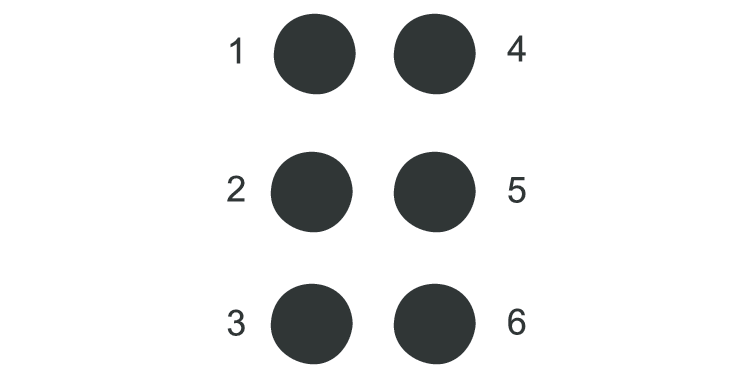
\includegraphics[width=0.5\textwidth]{Braille-six-dot-cell.png}
\caption{Braille Cell}
\label{fig:example}
\end{figure}


Braille is not a language in itself but rather a code that can be used to write any language. Each cell can be combined in various ways to form the letters of the alphabet, numbers, and other symbols. For example, the first ten letters of the alphabet are created using the top four dots of the Braille cell, while the remaining letters are formed by adding the fifth and sixth dots. Additionally, specific dot patterns are used to signify numbers and punctuation.

Braille literacy is crucial for the personal and educational development of individuals with visual impairments. It provides them with the means to access written information, pursue education, and engage in a wide range of professional activities. Moreover, it enhances their independence and ability to participate fully in society.

There are different grades of Braille, each serving a specific purpose. Grade 1 Braille, also known as uncontracted Braille, is a straightforward transcription where each Braille cell corresponds directly to an individual letter, number, or punctuation mark. It is often used for beginners who are just learning to read and write in Braille. Grade 1 alphabet and numbers is shown in figure 1.2. Grade 2 Braille, or contracted Braille, involves the use of contractions to represent common words or groups of letters, allowing for more efficient reading and writing. Contracted Braille is commonly used in books, signage, and other written materials to save space and make reading quicker. Figure 1.3 shows some of the most common words represented in grade 2.[13]

\renewcommand{\thefigure}{1.\arabic{figure}}

\begin{figure}[h]
\centering
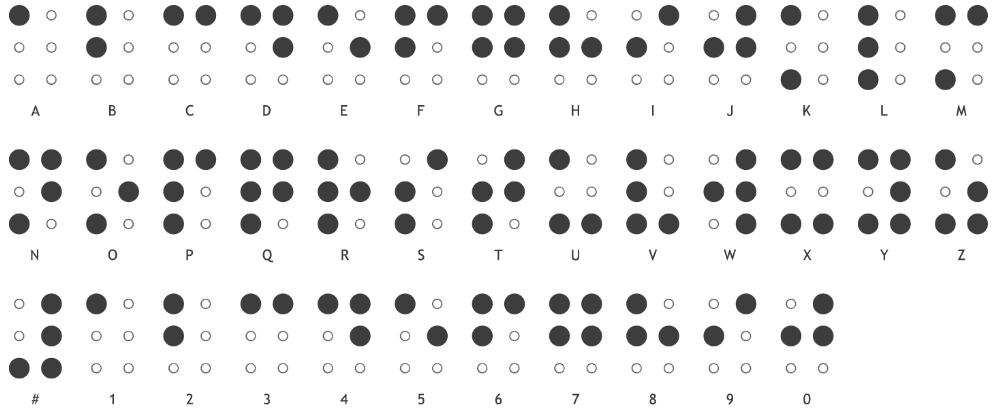
\includegraphics[width=0.9\textwidth]{alphabet_numbers.jpg}
\caption{Grade 1 Braille alphabet and numbers}
\label{fig:example}
\end{figure}

\begin{figure}[h]
\centering
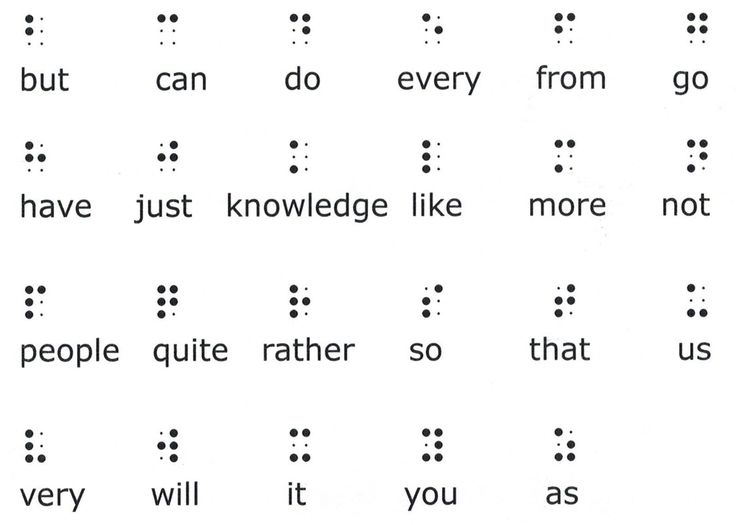
\includegraphics[width=0.6\textwidth]{grade2.jpg}
\caption{Common grade 2 Braille words}
\label{fig:example}
\end{figure}


Despite its importance, the availability of Braille materials is limited. Producing Braille books and resources is a complex and costly process, which contributes to the scarcity of accessible materials for the visually impaired. This lack of resources highlights the need for innovative solutions that can bridge the gap between Braille literacy and accessibility. Our project, the "Optical Braille Translator," aims to address this need by providing a system that translates Braille into English text and converts it into audible speech, thereby enhancing access to Braille content and supporting the literacy and independence of visually impaired individuals.

\subsection{Problem Statement}


Braille literacy is crucial for individuals with visual impairments, as it provides them with the ability to read and write independently. Despite its importance, the accessibility and usability of Braille materials pose some challenges. The primary problem this project addresses is that converting printed text into Braille or vice versa is a labor-intensive process. Moreover, individuals who are not proficient in Braille find it difficult to access Braille content. The accessibility of braille content to for everyone is so important. Braille language is the way visually impaired people would express themselves or their thought. It is the way to introduce their cultural production to the world.


Other challenges that further complicate the issue, as non-Braille users, including family members, educators, and caregivers, struggle to engage with Braille content, limiting the support they can offer to visually impaired individuals. The isolation experienced by those who rely on Braille due to the communication gap with non-Braille users highlights the need for inclusive solutions.

Additionally, students with visual impairments face difficulties in mainstream educational environments due to the scarcity of accessible Braille materials. Teachers without Braille proficiency are unable to provide adequate instructional support, impacting the quality of education for visually impaired students. 

A specific problem this project aims to solve is the correction of high school final exams for students using Braille. Exam papers must be transported to the capital for correction, risking partial or full damage during the journey. Moreover, the process involves individuals not knowledgeable enough about the academic content translating from Braille to text, followed by correction by another individual, which increases the probability of human errors. By addressing these issues, the project seeks to create a system that enhances the accessibility and usability of Braille materials, fostering greater inclusion and independence for individuals with visual impairments.

All the previous raises the need for a system that can make Braille content easily accessible to everyone, including those without Braille literacy skills.


\subsection{Project Overview}


Our project aims to solve this problem by developing a system that leverages image processing and deep learning techniques to facilitate the translation of scanned Braille images into English text. Additionally, the system converts the extracted text into audible speech, enhancing accessibility for visually impaired individuals. The project focuses on translating grade 1, front-only, scanned Braille images.

The system is designed to be user-friendly, ensuring that individuals with varying levels of technical expertise can use it effectively. Our project provides a solution that not only interprets Braille characters accurately but also synthesizes the extracted text into speech. This dual functionality makes Braille content more accessible and usable for a broader audience.

\subsubsection{Objectives}

The primary objective of our project is to develop a Braille to text translation system that can accurately detect and recognize Braille characters from scanned images using image processing and deep learning techniques. To further enhance the usability of the system, we aim to integrate a text-to-speech conversion feature that transforms the extracted English text into audible speech, making it accessible to individuals who cannot read Braille. Ensuring high accuracy and usability is another key objective, as we strive to design the system to achieve high accuracy in Braille recognition while providing a user-friendly interface for easy operation. Ultimately, the project seeks to enhance accessibility by enabling visually impaired individuals and those without Braille literacy skills to access Braille content effortlessly.

\subsubsection{Methodology}

To achieve these objectives, our project employs a multi-step approach. The scanned Braille images undergo preprocessing filters to enhance image quality and prepare the digital image for analysis. This step includes noise reduction, normalization, and page alignment. 



The system utilizes image processing techniques to detect Braille characters using two different methods: dot detection using Hough circle transformation(HCT) or detection of symbols using white spaces between the symbols and dividing the page to individual symbols. 

The next step is recognize the symbols using again two approaches: grid formation or using CNN to recognise the symbols from the divided image .

The recognized Braille characters are translated into English text, and a text correction module is employed to ensure the accuracy and coherence of the translated text. 

The corrected text is then converted into audible speech using a text-to-speech engine, providing an auditory output of the Braille content.

Finally, a graphical user interface (GUI) is developed to facilitate easy interaction with the system, and extensive testing is conducted to evaluate the system's performance and accuracy. Each of these steps will be explained in detail in the upcoming chapters.

\begin{figure}[!ht]
\centering
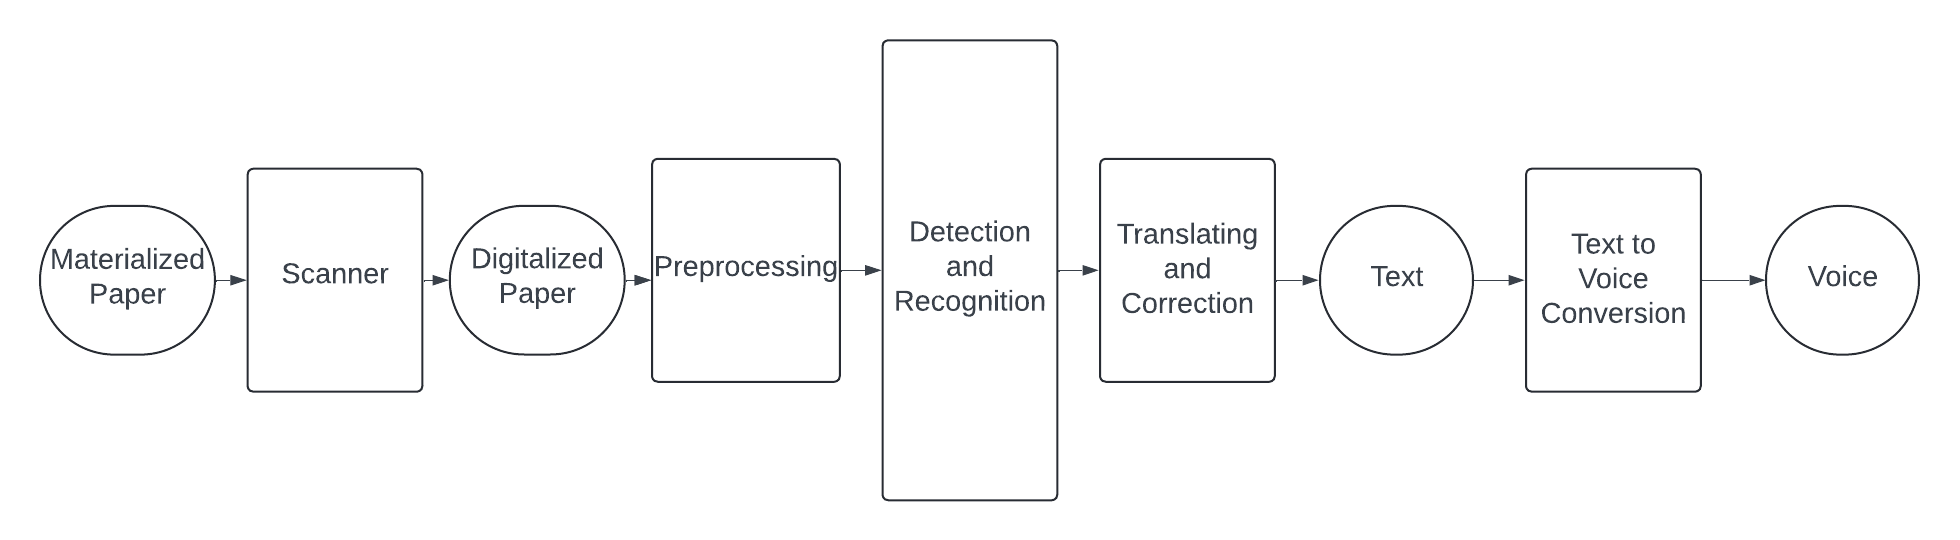
\includegraphics[width=1\linewidth]{Block diagram.png}
\caption{Block Diagram}
\label{fig:Block Diagram}
\end{figure} 

\subsubsection{Conclusion}

In conclusion, our project addresses a critical need in the realm of accessibility for visually impaired individuals. By combining image processing, deep learning, and text-to-speech technologies, we have developed a comprehensive solution that translates Braille into English text and converts it into audible speech. This innovative system not only enhances Braille literacy but also makes Braille content accessible to a wider audience, thereby bridging the gap between Braille literacy and accessibility.

The following chapters will delve into the technical details of the project, including the system design, preprocessing techniques, detection and recognition methods, and the implementation of text-to-speech conversion. Through this comprehensive exploration, we aim to provide a thorough understanding of the project's development and its impact on enhancing accessibility for visually impaired individuals.